% Options for packages loaded elsewhere
\PassOptionsToPackage{unicode}{hyperref}
\PassOptionsToPackage{hyphens}{url}
%
\documentclass[
]{article}
\usepackage{amsmath,amssymb}
\usepackage{iftex}
\ifPDFTeX
  \usepackage[T1]{fontenc}
  \usepackage[utf8]{inputenc}
  \usepackage{textcomp} % provide euro and other symbols
\else % if luatex or xetex
  \usepackage{unicode-math} % this also loads fontspec
  \defaultfontfeatures{Scale=MatchLowercase}
  \defaultfontfeatures[\rmfamily]{Ligatures=TeX,Scale=1}
\fi
\usepackage{lmodern}
\ifPDFTeX\else
  % xetex/luatex font selection
\fi
% Use upquote if available, for straight quotes in verbatim environments
\IfFileExists{upquote.sty}{\usepackage{upquote}}{}
\IfFileExists{microtype.sty}{% use microtype if available
  \usepackage[]{microtype}
  \UseMicrotypeSet[protrusion]{basicmath} % disable protrusion for tt fonts
}{}
\makeatletter
\@ifundefined{KOMAClassName}{% if non-KOMA class
  \IfFileExists{parskip.sty}{%
    \usepackage{parskip}
  }{% else
    \setlength{\parindent}{0pt}
    \setlength{\parskip}{6pt plus 2pt minus 1pt}}
}{% if KOMA class
  \KOMAoptions{parskip=half}}
\makeatother
\usepackage{xcolor}
\usepackage[margin=1in]{geometry}
\usepackage{color}
\usepackage{fancyvrb}
\newcommand{\VerbBar}{|}
\newcommand{\VERB}{\Verb[commandchars=\\\{\}]}
\DefineVerbatimEnvironment{Highlighting}{Verbatim}{commandchars=\\\{\}}
% Add ',fontsize=\small' for more characters per line
\usepackage{framed}
\definecolor{shadecolor}{RGB}{248,248,248}
\newenvironment{Shaded}{\begin{snugshade}}{\end{snugshade}}
\newcommand{\AlertTok}[1]{\textcolor[rgb]{0.94,0.16,0.16}{#1}}
\newcommand{\AnnotationTok}[1]{\textcolor[rgb]{0.56,0.35,0.01}{\textbf{\textit{#1}}}}
\newcommand{\AttributeTok}[1]{\textcolor[rgb]{0.13,0.29,0.53}{#1}}
\newcommand{\BaseNTok}[1]{\textcolor[rgb]{0.00,0.00,0.81}{#1}}
\newcommand{\BuiltInTok}[1]{#1}
\newcommand{\CharTok}[1]{\textcolor[rgb]{0.31,0.60,0.02}{#1}}
\newcommand{\CommentTok}[1]{\textcolor[rgb]{0.56,0.35,0.01}{\textit{#1}}}
\newcommand{\CommentVarTok}[1]{\textcolor[rgb]{0.56,0.35,0.01}{\textbf{\textit{#1}}}}
\newcommand{\ConstantTok}[1]{\textcolor[rgb]{0.56,0.35,0.01}{#1}}
\newcommand{\ControlFlowTok}[1]{\textcolor[rgb]{0.13,0.29,0.53}{\textbf{#1}}}
\newcommand{\DataTypeTok}[1]{\textcolor[rgb]{0.13,0.29,0.53}{#1}}
\newcommand{\DecValTok}[1]{\textcolor[rgb]{0.00,0.00,0.81}{#1}}
\newcommand{\DocumentationTok}[1]{\textcolor[rgb]{0.56,0.35,0.01}{\textbf{\textit{#1}}}}
\newcommand{\ErrorTok}[1]{\textcolor[rgb]{0.64,0.00,0.00}{\textbf{#1}}}
\newcommand{\ExtensionTok}[1]{#1}
\newcommand{\FloatTok}[1]{\textcolor[rgb]{0.00,0.00,0.81}{#1}}
\newcommand{\FunctionTok}[1]{\textcolor[rgb]{0.13,0.29,0.53}{\textbf{#1}}}
\newcommand{\ImportTok}[1]{#1}
\newcommand{\InformationTok}[1]{\textcolor[rgb]{0.56,0.35,0.01}{\textbf{\textit{#1}}}}
\newcommand{\KeywordTok}[1]{\textcolor[rgb]{0.13,0.29,0.53}{\textbf{#1}}}
\newcommand{\NormalTok}[1]{#1}
\newcommand{\OperatorTok}[1]{\textcolor[rgb]{0.81,0.36,0.00}{\textbf{#1}}}
\newcommand{\OtherTok}[1]{\textcolor[rgb]{0.56,0.35,0.01}{#1}}
\newcommand{\PreprocessorTok}[1]{\textcolor[rgb]{0.56,0.35,0.01}{\textit{#1}}}
\newcommand{\RegionMarkerTok}[1]{#1}
\newcommand{\SpecialCharTok}[1]{\textcolor[rgb]{0.81,0.36,0.00}{\textbf{#1}}}
\newcommand{\SpecialStringTok}[1]{\textcolor[rgb]{0.31,0.60,0.02}{#1}}
\newcommand{\StringTok}[1]{\textcolor[rgb]{0.31,0.60,0.02}{#1}}
\newcommand{\VariableTok}[1]{\textcolor[rgb]{0.00,0.00,0.00}{#1}}
\newcommand{\VerbatimStringTok}[1]{\textcolor[rgb]{0.31,0.60,0.02}{#1}}
\newcommand{\WarningTok}[1]{\textcolor[rgb]{0.56,0.35,0.01}{\textbf{\textit{#1}}}}
\usepackage{graphicx}
\makeatletter
\def\maxwidth{\ifdim\Gin@nat@width>\linewidth\linewidth\else\Gin@nat@width\fi}
\def\maxheight{\ifdim\Gin@nat@height>\textheight\textheight\else\Gin@nat@height\fi}
\makeatother
% Scale images if necessary, so that they will not overflow the page
% margins by default, and it is still possible to overwrite the defaults
% using explicit options in \includegraphics[width, height, ...]{}
\setkeys{Gin}{width=\maxwidth,height=\maxheight,keepaspectratio}
% Set default figure placement to htbp
\makeatletter
\def\fps@figure{htbp}
\makeatother
\setlength{\emergencystretch}{3em} % prevent overfull lines
\providecommand{\tightlist}{%
  \setlength{\itemsep}{0pt}\setlength{\parskip}{0pt}}
\setcounter{secnumdepth}{-\maxdimen} % remove section numbering
\usepackage{booktabs}
\usepackage{longtable}
\usepackage{array}
\usepackage{multirow}
\usepackage{wrapfig}
\usepackage{float}
\usepackage{colortbl}
\usepackage{pdflscape}
\usepackage{tabu}
\usepackage{threeparttable}
\usepackage{threeparttablex}
\usepackage[normalem]{ulem}
\usepackage{makecell}
\usepackage{xcolor}
\ifLuaTeX
  \usepackage{selnolig}  % disable illegal ligatures
\fi
\IfFileExists{bookmark.sty}{\usepackage{bookmark}}{\usepackage{hyperref}}
\IfFileExists{xurl.sty}{\usepackage{xurl}}{} % add URL line breaks if available
\urlstyle{same}
\hypersetup{
  pdftitle={Advanced Timber},
  pdfauthor={Franca Kaba Gómez},
  hidelinks,
  pdfcreator={LaTeX via pandoc}}

\title{Advanced Timber}
\author{Franca Kaba Gómez}
\date{2025-07-07}

\begin{document}
\maketitle

\hypertarget{introduction}{%
\subsection{Introduction}\label{introduction}}

Cameroon ranks as the fifth largest cocoa producer globally, with the
sector playing a significant role in the country's rural economy.
Production is predominantly carried out by smallholder farmers, whose
livelihoods are closely tied to cocoa cultivation. Introduced during the
German colonial period as a cash crop, cocoa has since become a
cornerstone of agricultural export in Cameroon. Compared to cocoa from
some neighboring countries, Cameroonian cocoa is often considered less
affected by pesticide residues, enhancing its appeal in increasingly
quality-conscious global markets. In recent years, producers have also
benefited from favorable world market prices.

Despite its economic significance, cocoa production in Cameroon faces
numerous structural and environmental challenges. The international
cocoa price remains highly volatile, exposing producers to significant
income uncertainty. Input costs can be prohibitively high in remote
rural areas, limiting farmers' ability to invest in yield improvements.
Agronomically, cocoa is highly sensitive to temperature fluctuations and
drought, and remains vulnerable to a range of pests and diseases, all of
which are exacerbated by climate change. Additionally, the sector is
hampered by supply chain inefficiencies, including poor infrastructure
and limited access to markets, while unsustainable expansion has
contributed to deforestation. These issues are further compounded by
sociodemographic pressures, such as aging farming populations, limited
access to education and extension services, and other inherent
constraints to smallholder farming systems.

Recent market trends, however, suggest that cocoa prices may
increasingly reflect the growing production risks associated with
climate variability, pest pressure, and land-use constraints.
Nonetheless, long-term global demand for cocoa is projected to rise
steadily, driven by sustained consumption in both emerging and
established markets. This continued demand underscores cocoa's strategic
importance not only as a global commodity but also as a source of
monetary income for otherwise predominantly subsistence-oriented
smallholder farmers. Cocoa is well-suited to agroforestry systems due to
its preference for shaded environments, offering opportunities for more
sustainable, biodiversity-friendly cultivation practices. Furthermore,
the presence of relatively well-established supply chains provides a
foundation for interventions aimed at improving value addition,
traceability, and farmer livelihoods.

One such improvement could be the introduction of timber trees, such as
Erythrophleum ivorense into cocoa plantations. Timber constitutes
another popular export product from Cameroon, which is predominantly
directed to the European and Chinese market. In Europe, however,
exporters of timber have to deal with regulations that aim to reduce
illegal logging activities. Trees from agroforestry plantations can thus
offer an opportunity for farmers to partake in the timber market in a
sustainable way.

\hypertarget{methodology}{%
\subsection{Methodology}\label{methodology}}

As a baseline, cocoa farming in a standard monoculture system on 2-6
hectares are considered. The integration would occur in a randomized
design with approximately 100-120 trees per hectare. The first harvest
of timber is anticipated after approximately 30 years, with the total
observed timeframe extending to 50 years. This long-term design allows
for the evaluation of both the establishment and maturation phases of
timber integration within an agroforestry context and can evaluate the
economic development of farms after the onset of economic returns from
farming activity. The model observes economical benefits of individual
smallholder farmers and does not consider ecological benefits or
benefits on a communal or regional scale.

In the cocoa monoculture system, farmer income is solely derived from
cocoa yield, which is influenced by labor inputs, agricultural inputs
(fertilizer, pesticides, and seedlings), and exposure to environmental
risks. Labor costs are disaggregated into full-time and part-time
employees, as well as family workforce contributions. Cocoa yield is
negatively affected by climatic and biotic stressors, particularly heavy
rainfall, drought, and pest and disease outbreaks. These risks represent
significant sources of yield variability and income instability. Market
prices, including the cocoa world market price and the farmer's Free on
Board (FOB) share, further mediate final cocoa income. In contrast, the
cocoa-timber agroforestry system integrates 120-200 timber trees per
hectare into existing cocoa plots. This diversified system introduces
additional cost categories, including timber establishment and
harvesting costs. Timber establishment costs encompass seedling
procurement, workforce for planting, and transport-related expenses such
as truck rental and gasoline. Timber harvesting involves further labor
and equipment costs. As in monoculture, labor and agricultural input
costs remain relevant. The agroforestry system generates dual income
streams from cocoa and timber. Timber income depends on timber yield and
farmgate prices, which are in turn influenced by factors such as tree
density and the physical characteristics of timber trees (height and
diameter). Cocoa income remains tied to cocoa yield and prices, as in
the monoculture system. 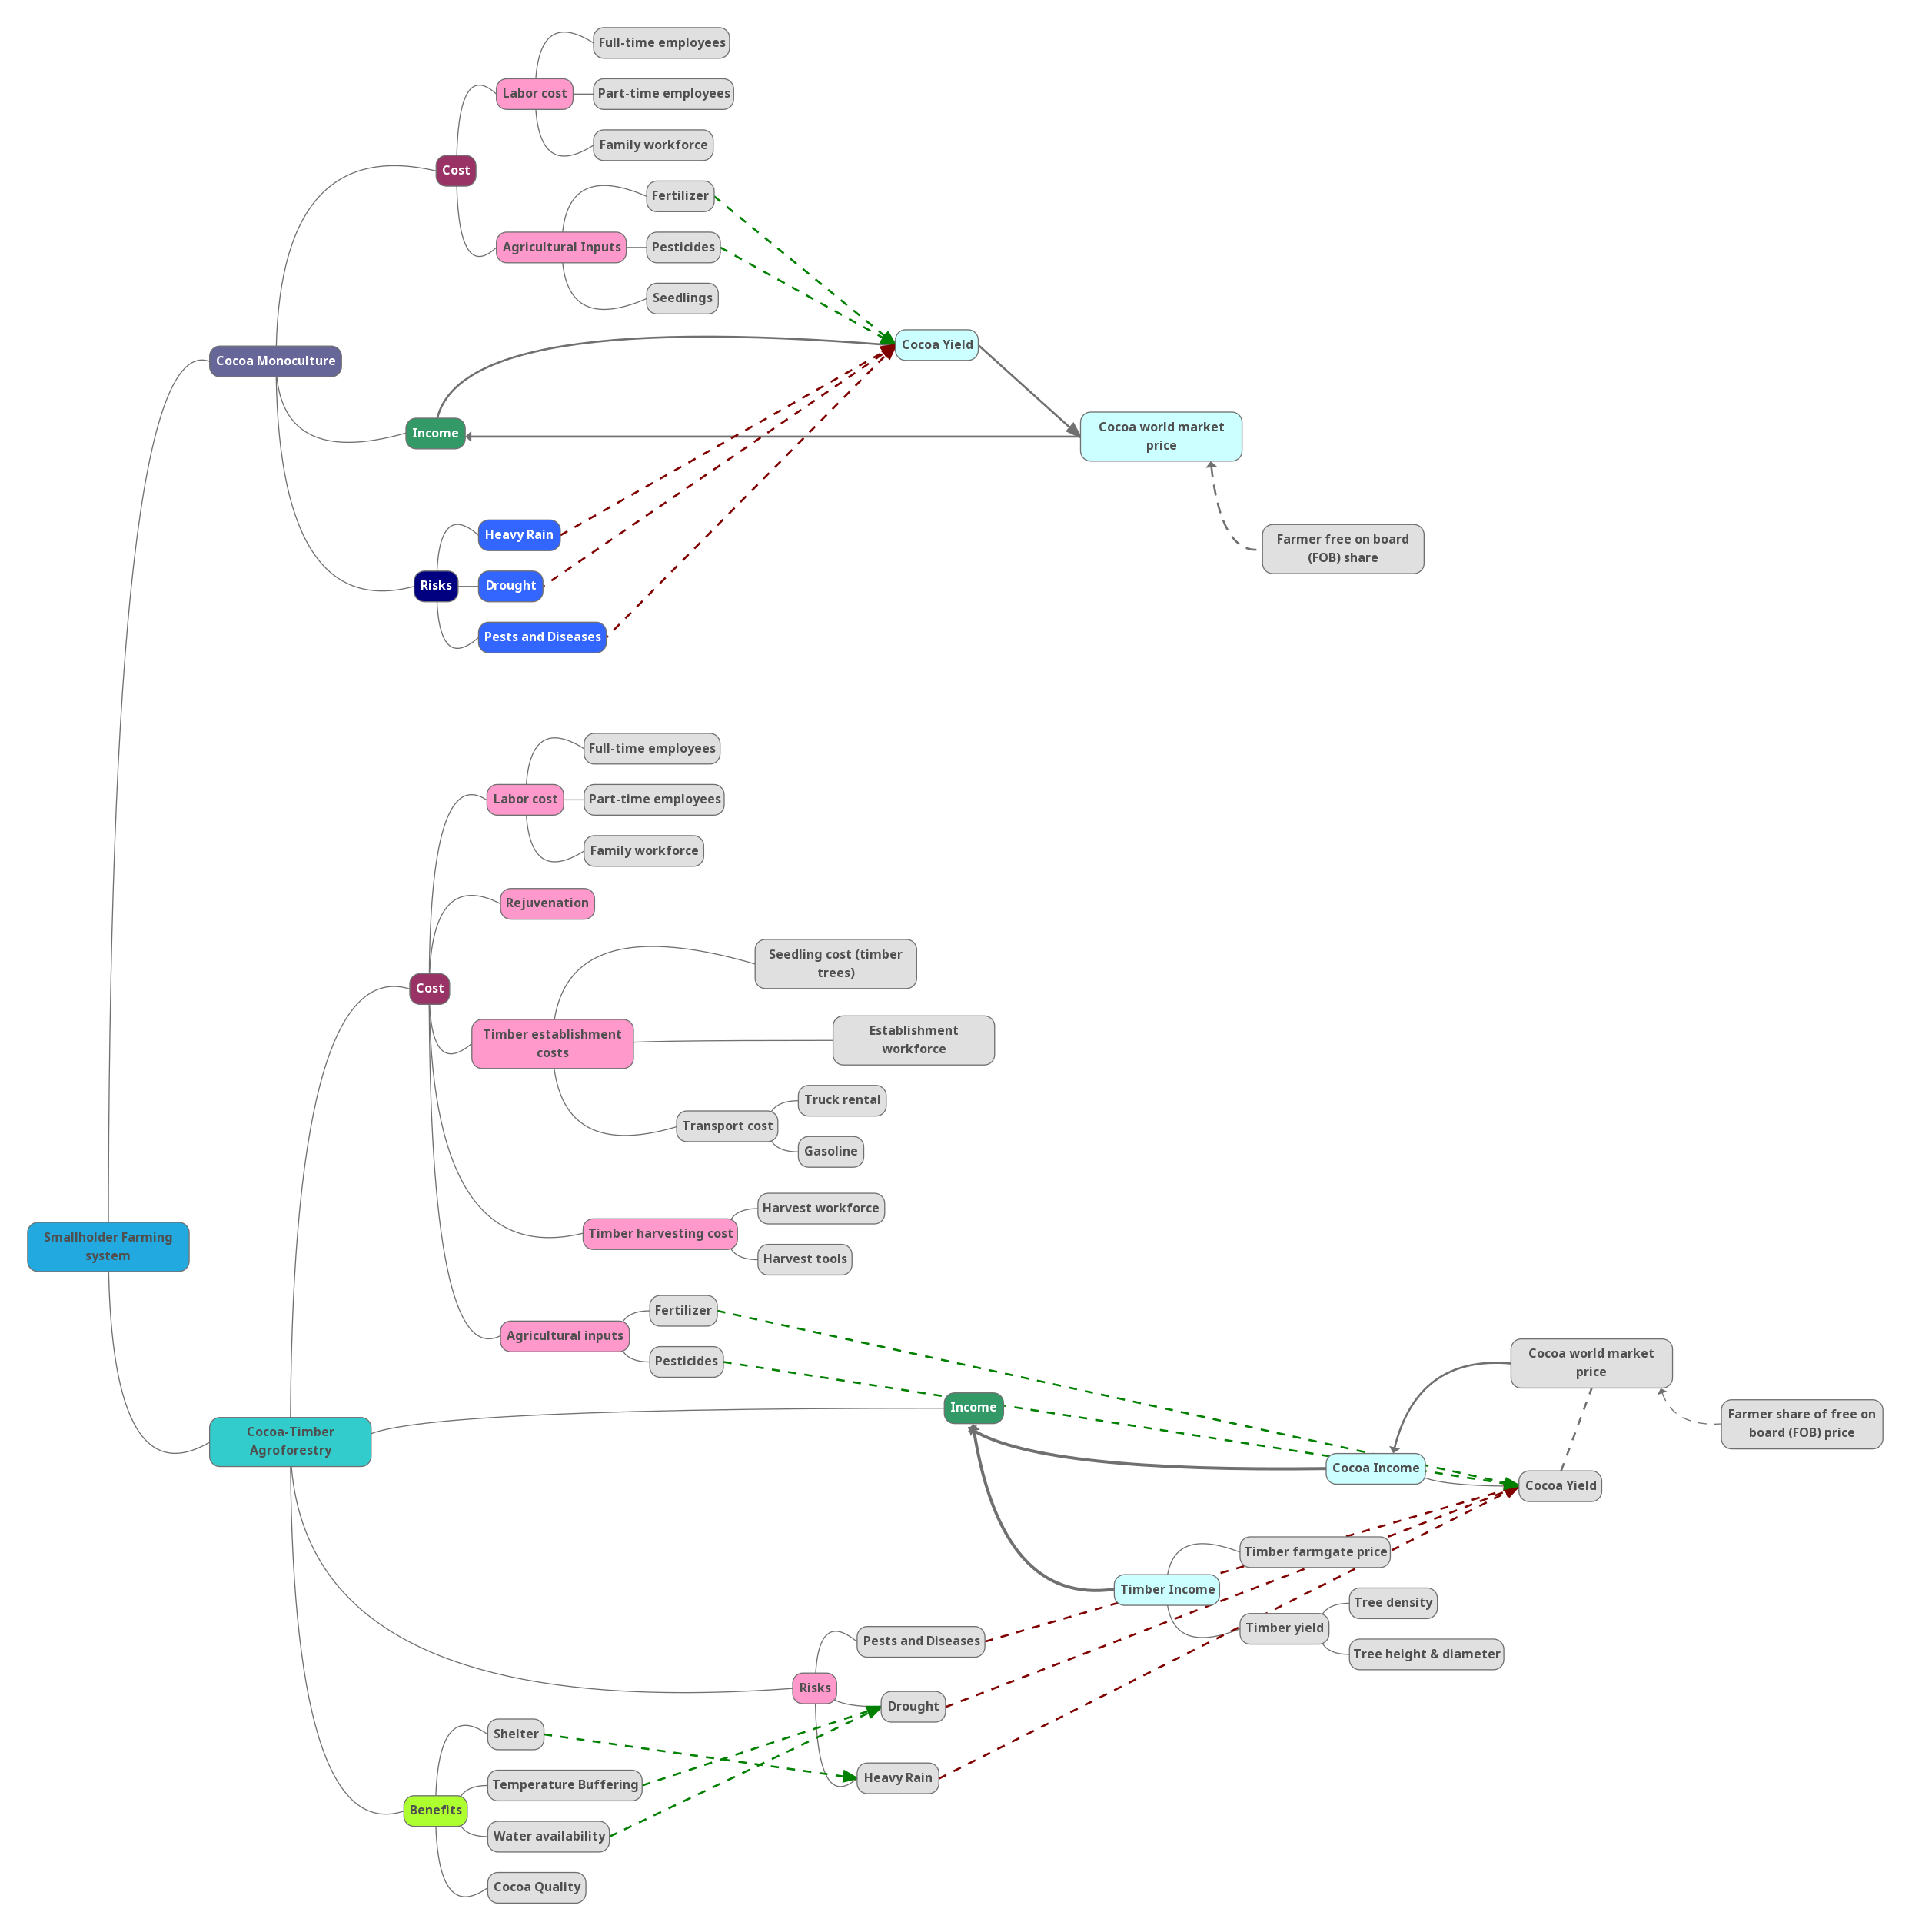
\includegraphics{Figure_1.png} Where applicable,
the above-mentioned factors were then estimated and set as variables.
Alternatively, variables that allowed the quantification of those
factors were identified and estimated. The estimations were mostly based
on literature, but some, namely farm size and yield, as well as
employment data were extracted from a survey carried out among 9 farmers
in the region of Cameroon Sud.This survey can be accessed
\href{https://docs.google.com/forms/d/1HqvVWuC2wZQChxLh2Mdu3DbTOk21pJ9Ffn6OML-6epw/edit\#responses}{here}
(Access from the authors may be required). It is important to mention
that any calculations considered the farm as a whole, and the model is
not fit to calculate either cost or profit per hectare. Table 1
summarizes the variables created for the decision model in this report.

\newpage

\begin{verbatim}
## Warning in styling_latex_scale(out, table_info, "down"): Longtable cannot be
## resized.
\end{verbatim}

\begin{longtable}[t]{lrlrlll}
\caption{\label{tab:table}Table 1: Variables used for the Model. Important Note: The Cocoa Price was defined 50 times to model cocoa price volatility. Price ranges 2-50 are not displayed here since they are identical.}\\
\toprule
Variable & lower & median & upper & distribution & description & source\\
\midrule
farm\_size & 2.0000 & NA & 6.000 & norm & Farm Size (ha) & https://forms.gle/n6US4VE7z6RhTqsH7\\
dry\_year\_incidence & 0.0010 & NA & 0.050 & tnorm\_0\_1 & Dry Year Incidence (probability) & World Bank Climate Change Knowledge Portal.\\
dry\_year\_damage & 0.3000 & NA & 0.600 & tnorm\_0\_1 & Dry Year Damage (yield loss fraction) & own estimation\\
dry\_year\_damage\_establishment & 1.0500 & NA & 1.200 & posnorm & additional damage during dry years in establishment phase & own estimation\\
dry\_year\_damage\_established & 0.4000 & NA & 0.900 & tnorm\_0\_1 & reduced damage during dry years by shading & own estimation\\
\addlinespace
heavy\_rainfall\_incidence & 0.1000 & NA & 0.400 & tnorm\_0\_1 & Heavy Rainfall Incidence (probability) & World Bank Climate Change Knowledge Portal.\\
heavy\_rainfall\_damage & 0.0500 & NA & 0.400 & tnorm\_0\_1 & Heavy Rainfall Damage (yield loss or multiplier) & own estimation\\
heavy\_rainfall\_damage\_established & 0.7000 & NA & 0.900 & tnorm\_0\_1 & reduced damage during heavy rain by throughpass/uptake/erosion protection & own estimation\\
cocoa\_pest\_and\_disease\_incidence & 0.8000 & NA & 0.900 & tnorm\_0\_1 & Cocoa Pest and Disease Incidence (probability) & Mahob et al. (2014)\\
cocoa\_pest\_and\_disease\_damage & 0.0500 & NA & 0.800 & tnorm\_0\_1 & Cocoa Pest and Disease Damage (yield loss fraction) & Mahob et al. (2014)\\
\addlinespace
labor\_price & 30000.0000 & NA & 60000.000 & norm & Labor Price (CFA/month/person) & ALIGN-Living Wage Cameroon. ANKER.\\
labor\_persons\_full\_time & 0.0000 & NA & 2.000 & norm & Full-time Labor (persons) & https://forms.gle/n6US4VE7z6RhTqsH7\\
labor\_persons\_seasonal & 1.0000 & NA & 5.000 & norm & Seasonal Labor (persons) & https://forms.gle/n6US4VE7z6RhTqsH7\\
fertilizer\_cost & 500.0000 & NA & 1000.000 & norm & Fertilizer Cost (CFA/kg) & facebook marketplace\\
fertilizer\_amount & 1.0000 & NA & 1.010 & norm & Fertilizer Amount (kg) & own estimation, Michel et. al. (2024)\\
\addlinespace
pesticide\_cost & 23000.0000 & NA & 35000.000 & norm & Pesticide Cost (CFA) & Mahob et al. (2014)\\
pesticide\_frequency & 5.0000 & NA & 15.000 & norm & Pesticide Frequency (treatments/year) & Mahob et al. (2014) and Michel et. al. (2024)\\
family\_labor & 1.0000 & NA & 3.000 & norm & Family Labor Cost (CFA/year) & ALIGN-Living Wage Cameroon. ANKER.\\
cocoa\_harvest & 150.0000 & NA & 4000.000 & norm & Cocoa Harvest (kg) & https://forms.gle/n6US4VE7z6RhTqsH7\\
cocoa\_price\_percent\_farmgate & 0.4500 & NA & 1.100 & norm & Farmgate Price Share (fraction of world price) & Laven, Buunk, and Ammerlaan (2016)\\
\addlinespace
pesticide\_effect & 1.0100 & NA & 1.028 & norm & pesticide efficiency & Bomdzele and Molua (2023)\\
fertilizer\_effect & 1.1000 & NA & 1.500 & norm & fertilizer effect on yield & own estimation\\
tree\_density & 120.0000 & NA & 200.000 & norm & density of trees on farm & own estimation\\
tree\_growth\_diam & 4.5000 & NA & 6.500 & norm & diameter growth per tree per year in mm & (Michel et. al., 2024)\\
tree\_growth\_height & 20.0000 & NA & 50.000 & norm & height increase per tree per year in cm & own estimation\\
\addlinespace
tree\_initial\_height & 150.0000 & NA & 200.000 & norm & tree height at time of planting & own estimation\\
tree\_initial\_diameter & 5.0000 & NA & 10.000 & norm & tree diameter at planting in cm & (Bosch, 2006)\\
tree\_survival\_rate & 0.7000 & NA & 0.900 & tnorm\_0\_1 & tree survival rate upon establishment & (Bosch, 2006)\\
tree\_price & 167700.0000 & NA & 279500.000 & norm & price that farmers could receive per m(3) at farmgate & Dwi Saputra et al. (2024)\\
tree\_seedlings & 2000.0000 & NA & 3000.000 & norm & price for seedlings & facebook marketplace,\\
\addlinespace
seedling\_and\_equipment\_transport & 80000.0000 & NA & 120000.000 & norm & price for transport and gas & facebook marketplace,\\
labor\_persons\_establishment & 5.0000 & NA & 10.000 & norm & personnel for establishment labor per ha &  ALIGN-Living Wage Cameroon. ANKER.\\
impact\_trees\_cocoa & 0.7000 & NA & 0.800 & tnorm\_0\_1 & yield reduction by timber trees to cocoa & Dwi Saputra et al. (2024)\\
impact\_trees\_cocoa\_establishment & 0.6000 & NA & 0.700 & tnorm\_0\_1 & yield reduction by timber trees to cocoa in establishment phase & Dwi Saputra et al. (2024)\\
harvest\_material & 150000.0000 & NA & 250000.000 & norm & material for harvest & facebook marketplace\\
\addlinespace
labor\_persons\_harvest & 5.0000 & NA & 10.000 & norm & personnel for harvest of timber & own estimation based on farm size and tree density\\
inflation\_rate\_cameroon & 2.0000 & NA & 7.500 & posnorm & cameroonian inflation rate estimated from data 2000-2030(forecast) & Statista (2025)\\
inflation\_rate\_world & 2.6000 & NA & 9.000 & posnorm & global inflation rate estimated from data 2000-2030(forecast) & Statista (2025) [2]\\
cocoa\_price\_world\_market\_1-50 & 278.1793 & NA & 3461.433 & norm & World Market Cocoa Price (CFA/kg) & Federal Reserve Bank of St. Luis (2025)\\
\bottomrule
\end{longtable}
\newpage

\hypertarget{intervention-modeling}{%
\subsubsection{Intervention modeling}\label{intervention-modeling}}

To compare the economic outcomes of cocoa monoculture with an
agroforestry system integrating timber, the R package decisionSupport
(Luedeling et al., 2019) was applied to perform a Monte Carlo
simulation. A model function was developed to incorporate yearly
cashflows over a 50-year period under two scenarios: (1) cocoa
monoculture and (2) cocoa-timber agroforestry. Both models incorporate
production risks (e.g., drought, heavy rainfall, pests), management
costs (e.g., labor, fertilizers, pesticides), and market uncertainties
(e.g., fluctuating cocoa and timber prices, inflation). For each model,
parameter uncertainty was captured using probabilistic input estimates
as explained above. The simulations included 1,000 iterations
(mcSimulation) per scenario. Agroforestry included a delayed income
stream from timber harvests starting at year 30, along with adjusted
risk impacts due to tree presence. Discounted and undiscounted net
cashflows were computed for both systems. Key outputs, such as net
present values (NPV) and yearly cashflows, were summarized and compared
using the Monte Carlo results. Distribution plots were generated with
plot\_distributions() to visualize the variability and outcomes across
simulations.\\
The simulation analysis was further extended by visualizing annual
discounted cashflows for both systems using the plot\_cashflow()
function, which displays the median values along with the 25--75\% and
5--95\% percentile ranges.\\
To assess the influence of uncertain parameters on model outcomes, a
multi-variable Expected Value of Perfect Information (EVPI) analysis was
conducted using the multi\_EVPI() function. Finally, correlations among
key input variables were examined using Pearson correlation coefficients
calculated from the Monte Carlo sample (mcSimulation) and visualized
with the ggcorrplot package.For that purpose, a correlation matrix was
provided as seperate .csv file.

\hypertarget{introduction-of-correlations}{%
\subsubsection{Introduction of
Correlations}\label{introduction-of-correlations}}

To explore the possibility to introduce relationships among key
agroforestry variables related to timber and cocoa production, a
correlation matrix was constructed. The matrix included nine variables:
fertilizer cost, fertilizer amount, pesticide cost, pesticide frequency,
cocoa harvest, tree density, seedling and equipment transport, harvest
material, and labor persons involved in harvest. Correlation
coefficients ranged from -0.5 to 1, reflecting both positive and
negative associations among the variables. The correlations were based
on own estimations of the author and relied on technical knowledge
gained during the project. Nevertheless, they are here used as showcase
example only. The correlation matrix was incorporated into a Monte Carlo
simulation framework using the mcSimulation function. The resulting
simulated data were visualized with ggcorrplot,

\hypertarget{results}{%
\subsection{Results}\label{results}}

\hypertarget{net-present-value-after-50-years}{%
\subsubsection{Net present value after 50
years}\label{net-present-value-after-50-years}}

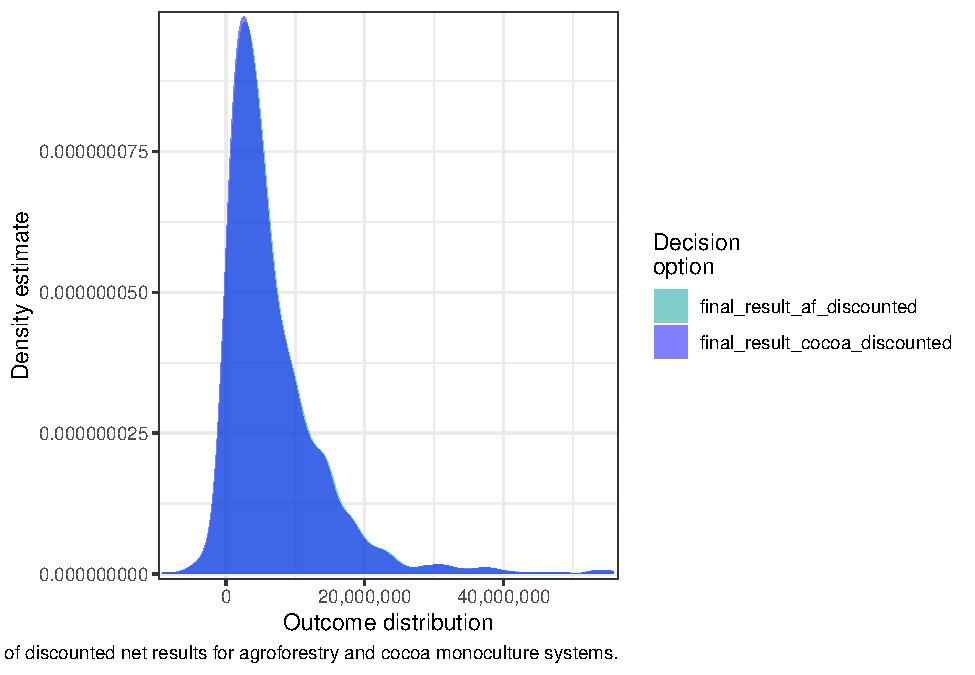
\includegraphics{Report_files/figure-latex/distibutions-1.pdf}

The generated plot shows the accumulated profit of both cocoa
monoculture and timber agroforestry. On first glance, the density
distributions of both systems are of similar shape, reaching from
\ensuremath{-8.439403\times 10^{6}} to
\ensuremath{4.9521781\times 10^{7}} in case of cocoa monoculture and
peaking at approximately 428 USD profit. With the intervention, the
distribution reaches from simulated scenarios of
\ensuremath{-8.28325\times 10^{6}} to
\ensuremath{4.9641979\times 10^{7}}and peaking at 428 USD profit
respectively. Concerning the risk of losses occurring after 50 years,
the density distribution of cocoa monoculture scenarios that return a
net profit \textless= 0 is 0.061, while the same risk to cocoa-timber
agroforestry is somewhat lower at 0.048.\\
Figure 2 plots the value of the decision, revealing that under all
circumstances, the expected value of decision is positive.

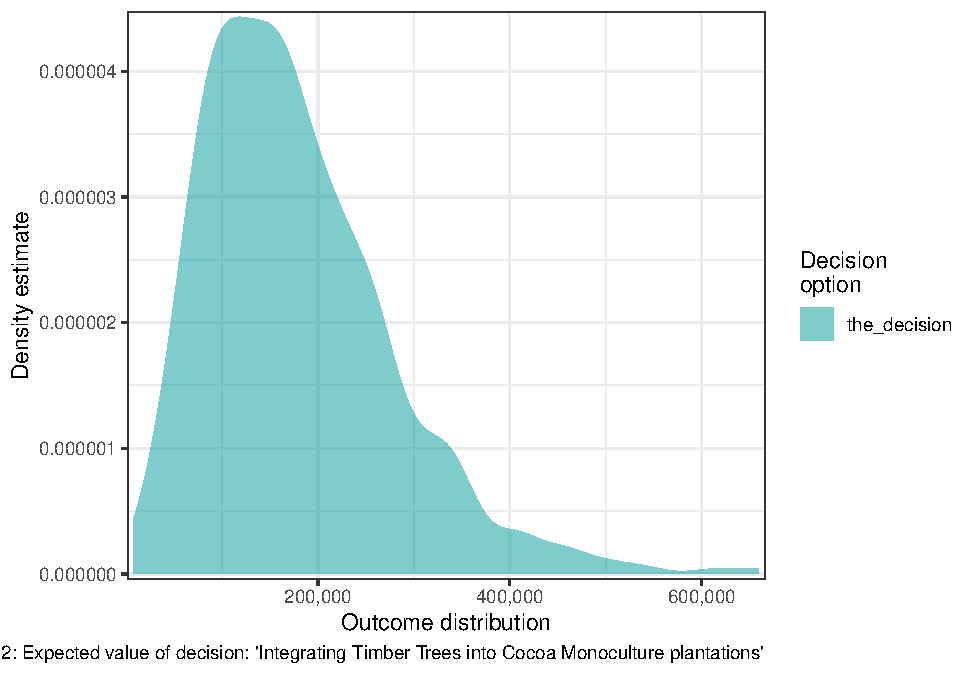
\includegraphics{Report_files/figure-latex/decision value-1.pdf}

\begin{Shaded}
\begin{Highlighting}[]
\NormalTok{peak\_index3 }\OtherTok{\textless{}{-}} \FunctionTok{which.max}\NormalTok{(mc\_simulation3[[}\StringTok{"y"}\NormalTok{]][[}\StringTok{"the\_decision"}\NormalTok{]])}
\NormalTok{max3}\OtherTok{\textless{}{-}}\FunctionTok{max}\NormalTok{(mc\_simulation3[[}\StringTok{"y"}\NormalTok{]][[}\StringTok{"the\_decision"}\NormalTok{]])}
\NormalTok{min3}\OtherTok{\textless{}{-}}\FunctionTok{min}\NormalTok{(mc\_simulation3[[}\StringTok{"y"}\NormalTok{]][[}\StringTok{"the\_decision"}\NormalTok{]])}
\end{Highlighting}
\end{Shaded}

The outcome density for the expected value of integrating timber
agroforestry into the cocoa plantation reaches from simulated returns of
-1907 to \ensuremath{7.49275\times 10^{5}}. It peaks at 397.

\hypertarget{cashflow}{%
\subsubsection{Cashflow}\label{cashflow}}

\textbf{Important note}: To display the variation of income flows, the
cashflow was plotted without discount over 50 years.

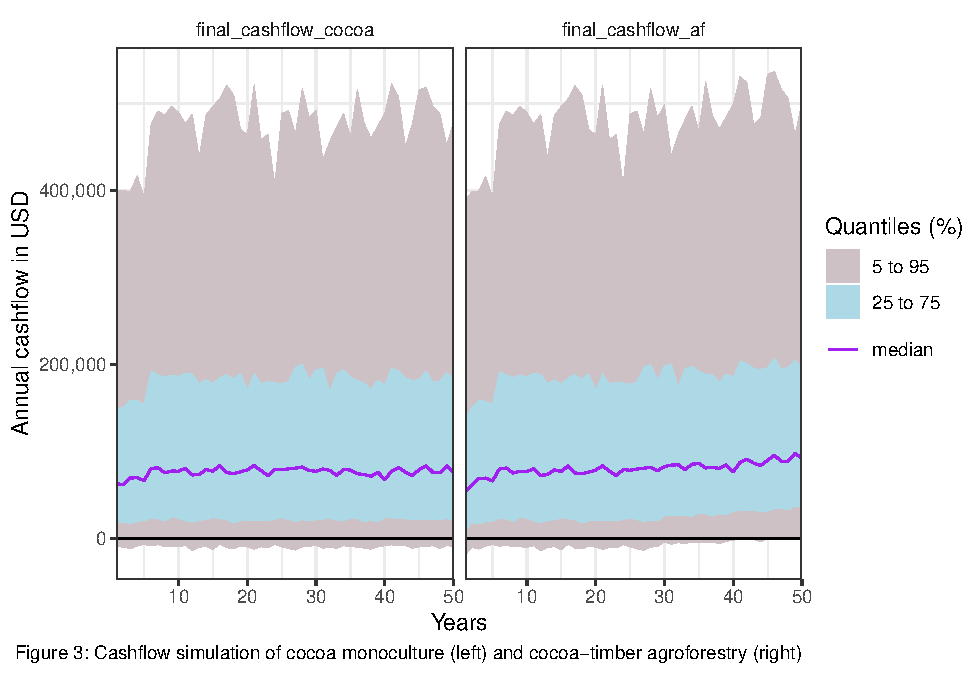
\includegraphics{Report_files/figure-latex/cashflows undiscounted-1.pdf}

Figure 3 compares the simulated annual cashflows for cocoa monoculture
(final\_cashflow\_cocoa) and cocoa-timber agroforestry
(final\_cashflow\_af). Both systems exhibit similar overall
distributions, with wide uncertainty ranges spanning the 5th to 95th
percentiles, reflecting inherent variability in market and production
conditions. The median cashflow trajectory (purple line) for the
agroforestry system starts at a lower point, but raises quickly and
appears slightly higher than that of the monoculture from approximately
year 10 onward, suggesting marginal long-term financial benefits
associated with the diversified system. Notably, the interquartile range
(25th to 75th percentile, lavender-blue area) is consistently wider in
both systems, indicating substantial variation in expected outcomes
across the simulation runs. However, the agroforestry system maintains
slightly higher medians with no marked increase in downside risk. This
combination results in 5th to 95th percentiles that seldomly reach below
0 from year 30, while this range reaches below 0 frequently in the cocoa
monoculture plot.

\#\#Value of information report

\begin{verbatim}
## [1] "Processing 1 output variables. This can take some time."
## [1] "Output variable 1 (mc_simulation3...y......final_result_cocoa_discounted...) completed."
\end{verbatim}

\begin{verbatim}
## Warning: There are no variables with a positive EVPI. You probably do not need
## a plot for that.
\end{verbatim}

\begin{verbatim}
## [1] "Processing 1 output variables. This can take some time."
## [1] "Output variable 1 (final_result_af) completed."
\end{verbatim}

\begin{verbatim}
## Warning: There are no variables with a positive EVPI. You probably do not need
## a plot for that.
\end{verbatim}

\begin{verbatim}
## [1] "Processing 1 output variables. This can take some time."
## [1] "Output variable 1 (mc_simulation3...y......the_decision...) completed."
\end{verbatim}

\begin{verbatim}
## Warning: There are no variables with a positive EVPI. You probably do not need
## a plot for that.
\end{verbatim}

The expected value of perfect information for all scenarios (cocoa
monoculture, cocoa-timber agroforestry and the decision) is zero, which
implies that in these simulations there is no variable that has enough
influence on the final result to be worth investigating more.

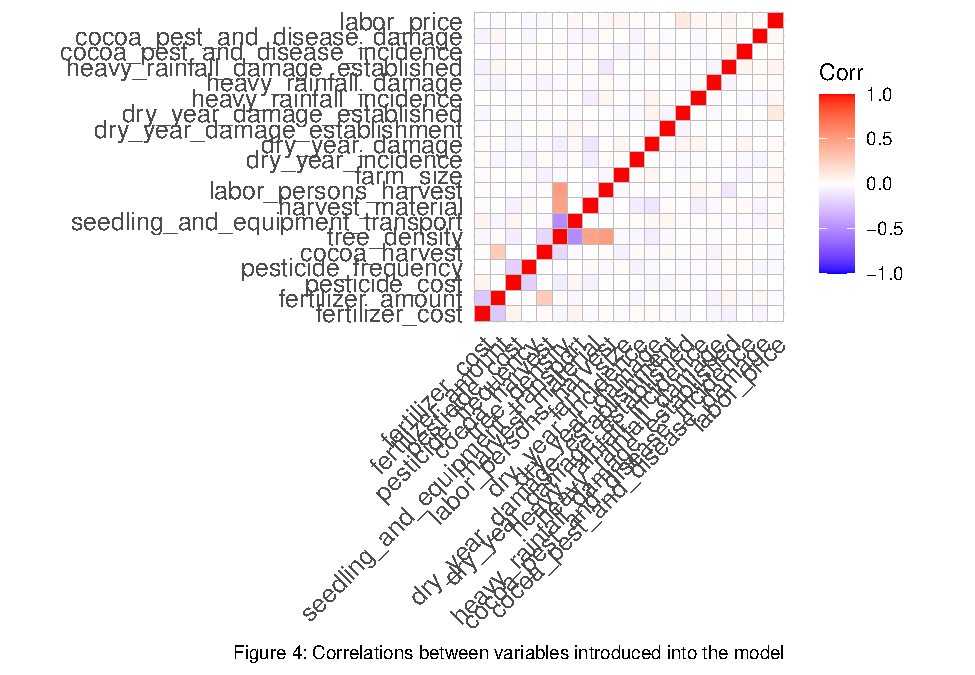
\includegraphics{Report_files/figure-latex/correlation-1.pdf}

The correlation plot shows that correlations could successfully be
forced into the simulation. Furthermore, it depicts some very small
correlations between variables that are not present in the decision
matrix, most likely due to random occurrances in model runs.

\begin{Shaded}
\begin{Highlighting}[]
\NormalTok{distribution\_plot\_corr}\OtherTok{\textless{}{-}}\FunctionTok{plot\_distributions}\NormalTok{(}
  \AttributeTok{mcSimulation\_object =}\NormalTok{ correlation,}
  \AttributeTok{vars =}\FunctionTok{c}\NormalTok{(}\StringTok{"final\_result\_af\_discounted"}\NormalTok{, }\StringTok{"final\_result\_cocoa\_discounted"}\NormalTok{),}
  \AttributeTok{method =} \StringTok{"smooth\_simple\_overlay"}\NormalTok{)}
\NormalTok{decision\_plot\_corr}\OtherTok{\textless{}{-}}\FunctionTok{plot\_distributions}\NormalTok{(}
  \AttributeTok{mcSimulation\_object =}\NormalTok{ correlation,}
  \AttributeTok{vars =}\FunctionTok{c}\NormalTok{(}\StringTok{"the\_decision"}\NormalTok{),}
  \AttributeTok{method =} \StringTok{"smooth\_simple\_overlay"}\NormalTok{)}
\NormalTok{cashflow\_correlation}\OtherTok{\textless{}{-}}\FunctionTok{plot\_cashflow}\NormalTok{(}\AttributeTok{mcSimulation\_object =}\NormalTok{ correlation, }\AttributeTok{cashflow\_var\_name =} \FunctionTok{c}\NormalTok{(}\StringTok{"final\_cashflow\_cocoa"}\NormalTok{, }\StringTok{"final\_cashflow\_af"}\NormalTok{),  }\AttributeTok{x\_axis\_name =} \StringTok{"Years"}\NormalTok{,}
              \AttributeTok{y\_axis\_name =} \StringTok{"Annual cashflow in USD"}\NormalTok{,}
              \AttributeTok{color\_25\_75 =} \StringTok{"lightblue"}\NormalTok{, }\AttributeTok{color\_5\_95 =} \StringTok{"lavenderblush3"}\NormalTok{,}
              \AttributeTok{color\_median =} \StringTok{"purple"}\NormalTok{)}
\NormalTok{plots}\OtherTok{\textless{}{-}}\NormalTok{distribution\_plot\_corr}\SpecialCharTok{/}\NormalTok{ decision\_plot\_corr }\SpecialCharTok{/}\NormalTok{cashflow\_correlation}
\NormalTok{correlation\_plot}\SpecialCharTok{+}\FunctionTok{labs}\NormalTok{(}\AttributeTok{caption =} \StringTok{"Figure 5: Density distributions in correlation plot"}\NormalTok{)}
\end{Highlighting}
\end{Shaded}

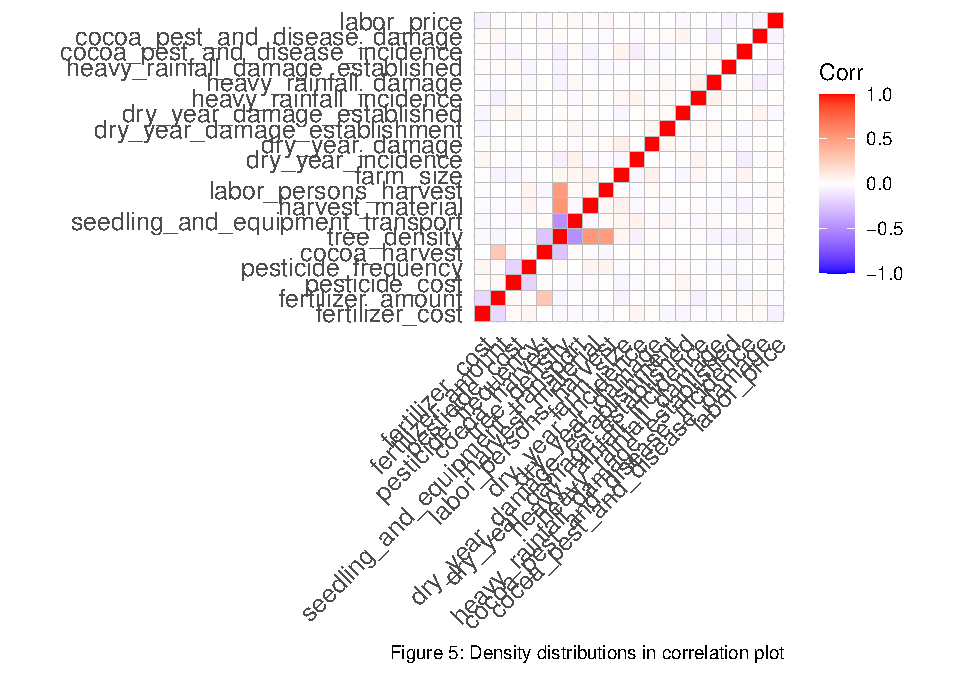
\includegraphics{Report_files/figure-latex/unnamed-chunk-2-1.pdf} Figure
5 displays the analytical plots from the model with integrated
correlations. There are only small differences between those and the
original plots. Due to the fragile nature of the correlation
estimations, they will not be discussed further in the scope of this
report.

\#\#Discussion

\end{document}
